

\documentclass[../../e3_tp2_main.tex]{subfiles}

\begin{document}
\chapter{Ejercicio 8}

Se propuso el diseño de un circuito que permita medir distancias utilizando un sensor ultrasónico de distancia (hc-sr04).
\par El circuito debe cumplir con los siguientes requerimientos: 
\begin{itemize}  
\item trigger, pin de entrada que dispara la medición en el flanco positivo. 
\item trigger enable, pin de entrada que habilita la señal de disparo.
\item meas, 8 bits de salida que indican el tiempo medido en unidades de 100 $\micro s$.
\item meas ready, pin de salida que indica que la medición ha finalizado. 
\end{itemize}

\section{Sensor HC-SR04}

El sensor de distancia hc-sr04
\footnote{Datasheet del sensor, Mouser.com. (2018). [online] Available at: https://www.mouser.com/ds/2/813/HCSR04-1022824.pdf [Accessed 13 Oct. 2018].}
 es un sensor de distancia ultrasónico. Posee cuatro terminales, dos de alimentación ($V_{cc}$y gnd), trigger y echo.
\par El terminal de trigger, acciona la medición, para ello se debe cambiar el estado del terminal a high por más de 10 $\micro s$, de esta manera el sensor comienza a medir. Luego por el pin de echo se devuelve un pulso de ancho T $\micro s$.
 El pulso devuelto es proporcional a  la distancia medida, Distancia = $ \frac {\micro s}{58}[cm]$.
\par El rango de medición del sensor es de 2cm a 4 metros. Por ende el ancho del pulso devuelto por echo es de entre 116 $\micro s$ y 23200$\micro s$.
\begin{figure}[H]	
	\centering
	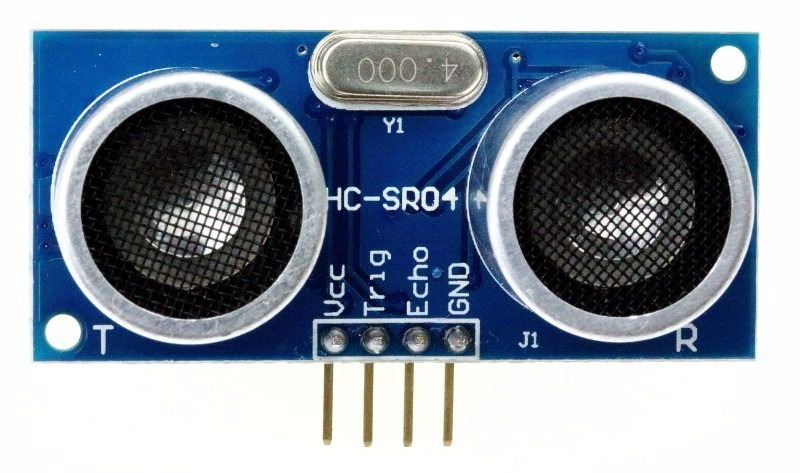
\includegraphics[width=0.4\textwidth]{imagenes/sensor.jpg}
	\caption{Sensor de distancia}
\end{figure}

\begin{figure}[H]	
	\centering
	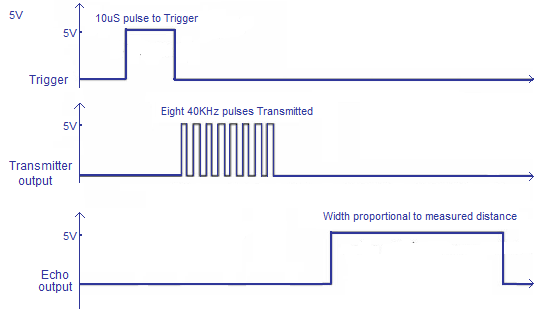
\includegraphics[width=0.45\textwidth]{imagenes/sensor_t.png}
	\caption{Diagrama temporal}
\end{figure}

\section{Circuito Implementado}

Se modularizó el circuito de la siguiente manera:
\begin{figure}[H]	
	\centering
	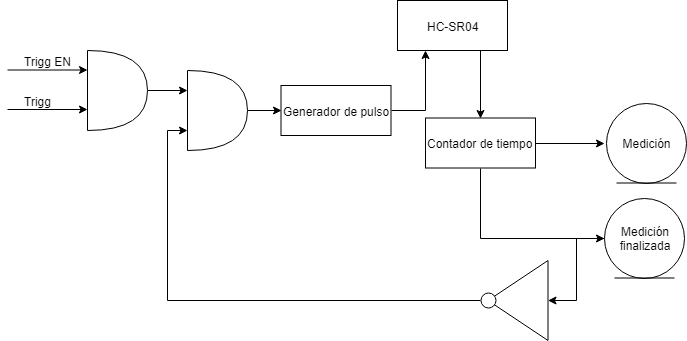
\includegraphics[width=0.5\textwidth]{imagenes/dBloques.png}
	\caption{Diagrama de bloques}\label{fig:dBloques}
\end{figure}
Los dos módulos principales, tal como se muestra en la imagen \ref{fig:dBloques}, son el generador de pulso y el contador de tiempo.
\par El generador de pulso, cuando recibe un flanco positivo, genera un pulso mayor a 10 $\micro s$ para que el sensor comience a medir.
\par El contador de tiempo, mide el ancho del pulso devuelto por echo, y lo devuelve en 8 bits, también se encarga de indicar que la medición finalizo.

\subsection{Generador de pulso}
El generador de pulso se implementó con un LM555. EL circuito utilizado fue el de la figura \ref{fig:555c}, dicho circuito genera un pulso de ancho$= R_a C 1.1$ s, para generar el disparo se debe generar un pulso menor que el configurado.
\par Como el sensor requiere un ancho de pulso mayor de 10$\micro s$, se eligieron los componentes para un pulso de 50$\micro s$, por ende el capacitor $C=10nf$ y $R_a=5k \Omega$

\begin{figure}[H]	
	\centering
	
\includegraphics[width=0.3\textwidth]{imagenes/555C.png}
	\caption{Circuito del generador de pulsos}\label{fig:555c}
\end{figure}
Para evitar que al generador de pulso, le ingrese una señal mayor a 50$\micro s$ se le coloco a la entrada (disparo) un RC con tiempo característico de 10$\micro s$. 

\subsection{Contador de tiempo}
Para medir cuanto tiempo el pulso de echo estuvo en high, se utilizó un contador de 8 bits y una señal cuadrada de 50 \% duty cycle como clock.
\par El contador utilizado, cuenta flancos positivos de clock. Por ende para contar cuanto tiempo la señal de echo estuvo en high, se conectó la entrada de clock del contador, a la salida de una AND. Las entradas de la AND son la señal de echo y una señal cuadrada de 10KHz. De esta manera, cada vez que ocurre un flanco de clock y la señal echo esta en high el contador incrementa en una unidad. Debido a que la frecuencia de la señal cuadrada es de 10Khz, cada unidad en el contador representa 100 $\micro s$.
\begin{figure}[H]	
	\centering
	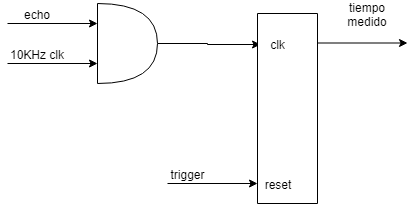
\includegraphics[width=0.5\textwidth]{imagenes/contador.png}
	\caption{Contador de tiempo}
\end{figure}
\par En cuanto al reset del contador se lo conecto al trigger del sensor, de esta manera, cada vez que se dispare una medición el contador vuelve a cero.
\subsection{OK meas}

En cuanto a la salida de ok meas, vasto con negar la señal de echo. Debido a que mientras no haya medición, la señal de echo se mantiene en low y por ende ok meas se mantiene en high. Cuando echo está en high, quiere decir que se está midiendo, y ok meas se encuentra en low.
\subsection{Prototipo}
Previo al diseño final del circuito, se decidió construir un prototipo del mismo en protoboard, para así probar el correcto funcionamiento de cada etapa y del conjunto. 
\begin{figure}[H]	
	\centering
	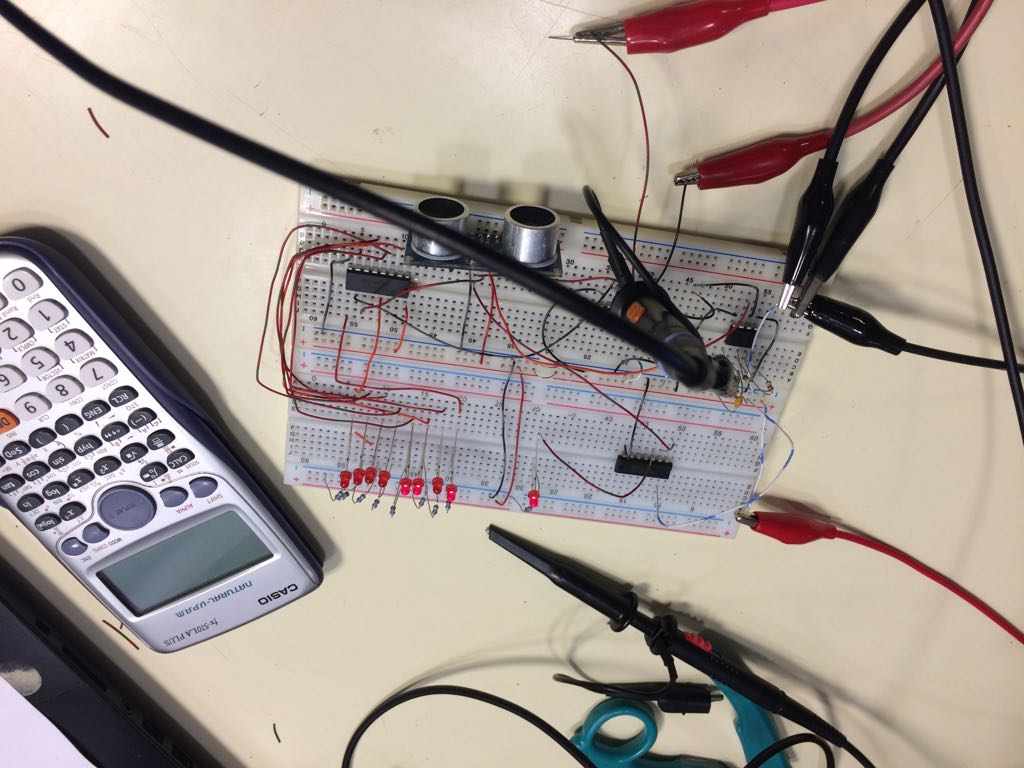
\includegraphics[angle=180,width=0.5\textwidth]{imagenes/prototipo.jpeg}
	\caption{Prototipo del circuito}
\end{figure}
Como el prototipo funciono correctamente, tal como se muestra en el siguiente link (https://youtu.be/xzRgiA1r85w). Se procedió al armado de la placa.
\subsection{Circuito}

El circuito final construido posee las siguientes características:
Entrada de trigger, trigger enable y clock. El clock al que se lo debe conectar es de 10Khz (señal cuadrada, 5v de amplitud y 50 \% de duty cycle).
Salida 8 bits que indican el tiempo medido, y 1 bit que indica que la medición finalizo.
\todo{sacar foto a la placa terminada y ponerla aca}.
\begin{figure}[H]	
	\centering
	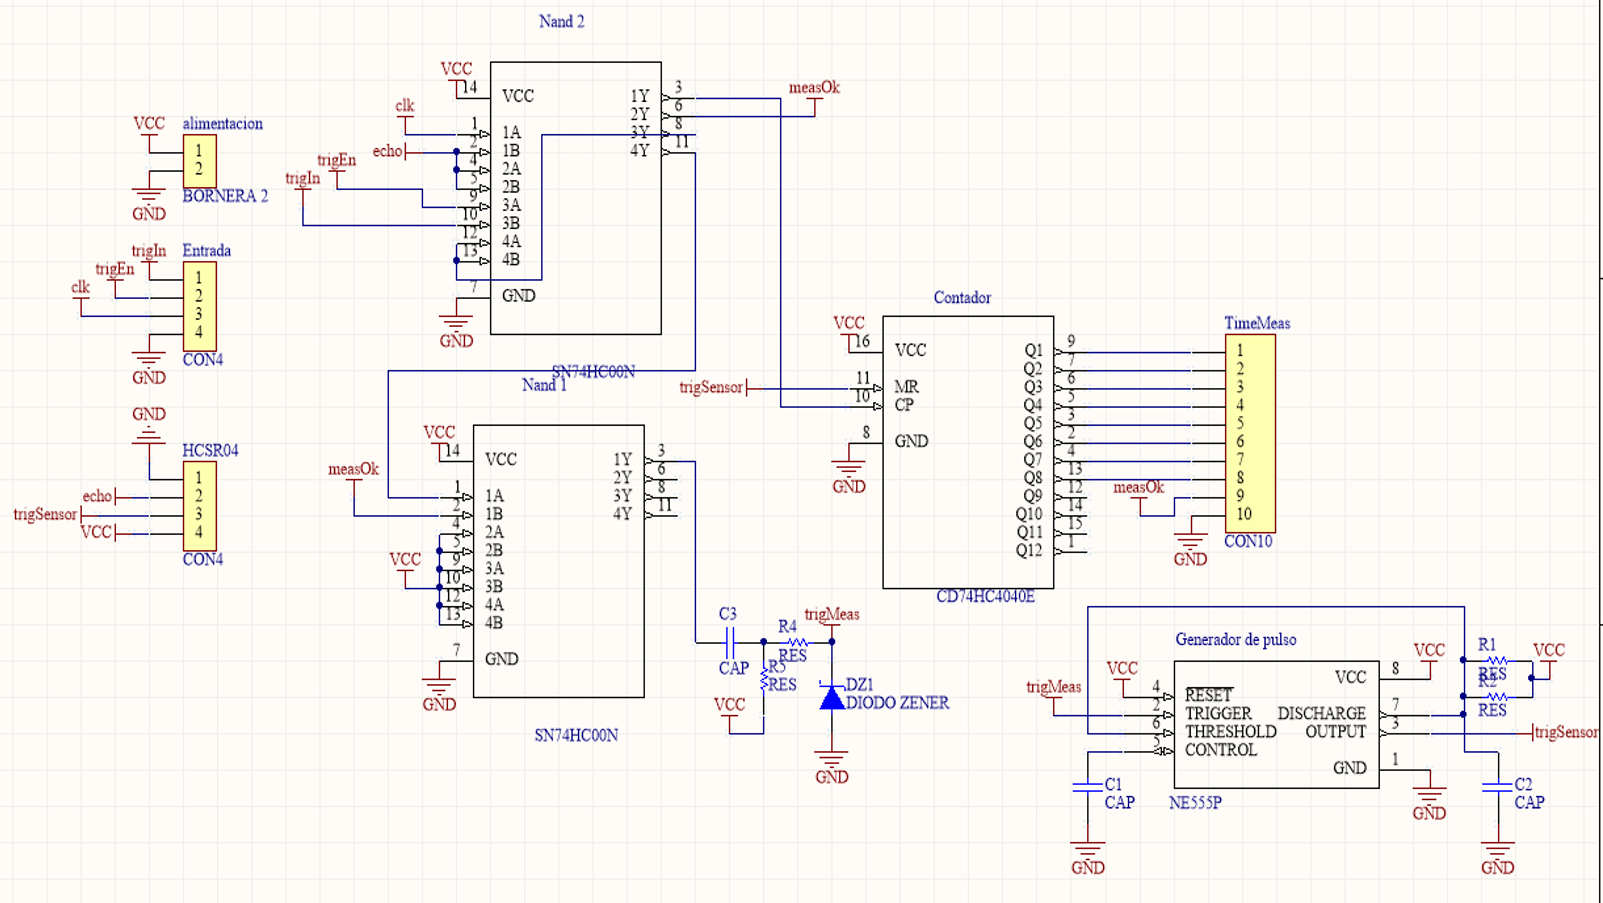
\includegraphics[width=0.5\textwidth]{imagenes/esquematico.png}
	\caption{Esquematico}
\end{figure}




\end{document}
